\documentclass[a4paper,12pt]{article}
\usepackage{amsfonts}
\usepackage{amssymb}
\usepackage{latexsym}
\usepackage{amsmath}
\usepackage{amsthm}
\usepackage{graphicx}
\usepackage{indentfirst}
\usepackage[polish]{babel}
\usepackage[T1]{fontenc}
\usepackage{polski}
\usepackage[utf8]{inputenc}
\usepackage[cp1250]{inputenc} % tu mo¿e byæ konieczne zast¹pienie "cp1250" przez np. "utf8"
\usepackage{array}
\usepackage{multirow}
\usepackage{geometry}
\geometry{hdivide={2cm,*,2cm}}
\geometry{vdivide={2cm,*,2cm}}
\usepackage{titlesec}
\usepackage{multicol}
\usepackage{caption}
\titlespacing{\section}{0ex}{1ex}{1ex} % zmniejszenie odstêpów przed i po tytule rozdzia³u...
\titleformat*{\section}{\sf\large\bfseries} % i zmiana kroju czcionki
\titlespacing{\subsection}{0ex}{0.75ex}{0.75ex} % % j/w dla tytu³ów podrozdzia³ów
\titleformat*{\subsection}{\sf\bfseries}

% Zmniejszenie odstêpów przed i za wzorami wystawionymi
\AtBeginDocument{
\addtolength{\abovedisplayskip}{-1ex}
\addtolength{\abovedisplayshortskip}{-1ex}
\addtolength{\belowdisplayskip}{-1ex}
\addtolength{\belowdisplayshortskip}{-1ex}
}
% Kilka przydatnych definicji
\newcolumntype{C}[1]{>{\centering\arraybackslash}m{#1}}
\newcommand{\razy}{\hspace{-0.5ex}\times\hspace{-0.5ex}} % mo¿e siê przydaæ


\begin{document}

\def\tablename{Tabela} % bez tej linii nazw¹ tabeli by³aby "Tablica"


\noindent
\textbf{Marcin Skrzypczak, 320735, grupa 5, projekt 1, zadanie 36}

\section*{Wstęp}
    Raport poświęcony jest przybliżaniu wartości całek podwójnych zadanych nad kołem jednostkowym, przy użyciu transformacji na współrzędne biegunowe oraz złożonej kwadratury prostokątów z punktem środkowym. Znaczącym zagadnieniem jest oszacowanie błędu metody, stąd testy zostały poświęcone badaniu tego zagadnienia. Badana metoda wyróżnia się prostotą implementacji, ale również niskim rzędem oraz często problematycznym rozkładem węzłów kwadratury. W ostatniej części zostaną zaproponowane metody minimalizacji błędu przybliżenia w stosunku do złożoności obliczeniowej.

\section*{Opis metody}
    Obszar całkowania zostaje zmieniony z $B_1=\{(x, y)\in R^2: x^2+y^2\leq 1 \}$ na $B_2 = \{(r, \phi): r=\sqrt{x^2+y^2}, \phi=\arctan(\frac{y}{x}), (x,y)\in B_1 \}$. Jakobian tej transformacji wynosi $r$, stąd:
    \[ \iint \limits_{B_1}f(x,y)dxdy = \iint \limits_{B_2}r f(r\cos{\phi},r\sin{\phi})drd\phi \]
    \\
    Kwadratura prostokątów z punktem środkowym przybliża całkę w następujący sposób:
    \[\int\limits_a^bf(x)dx\approx\sum\limits^N_{k=1}(x_k-x_{k-1})f\left(\frac{x_k+x_{k+1}}{2}\right),\]
    gdzie $x_0, x_1, ..., x_n$ są punktami podziałów przedziału całkowania, przy czym $x_0=a$ oraz $x_n=b$, a $N$ to liczba podziałów całkowanego przedziału.
    Kwadratura zostaje kolejno zastosowana względem modułu i argumentu.
    

\section*{Eksperymenty numeryczne}
    Metoda z pewną dokładnością przybliża wielomiany niższego stopnia, jednak już przy stopniu drugim, otrzymujemy duży błąd względny, który nie pozwala na zastosowanie jej w wielu przypadkach. Zwiększanie ilości węzłów jest jedyną możliwością zmniejszenia błędu, jednak nie jest to najbardziej efektywne, aby osiągnąć błąd rzędu $1e-10$, należy użyć ponad $1e6$ węzłów.
\begin{table}[h]
\centering
\begin{tabular}{|c|c|c|c|}
\hline
Funkcja              & Wartość dokładna & Wartość przybliżona & Błąd     \\ \hline
1                    & 3.1416           & 3.1416              & 0        \\ \hline
x                    & 0                & 0                   & 1,05e-16 \\ \hline
y                    & 0                & 0                   & 5,75e-17 \\ \hline
xy                   & 0                & 0                   & 6,10e-18 \\ \hline
x\textasciicircum{}2 & 0,7815           & 0,7854              & 3,93e-03 \\ \hline
y\textasciicircum{}2 & 0,7815           & 0,7854              & 3,93e-03 \\ \hline
x\textasciicircum{}4 & 0,3878           & 0,3927              & 4,89e-03 \\ \hline
y\textasciicircum{}4 & 0,3878           & 0,3927              & 4,89e-03 \\ \hline
\end{tabular}
\caption{Błąd metody, przy oparciu kwadratury na 100 węzłach}
\end{table}

\break

    Uśredniony błąd przy obliczaniu całek 4 stopnia wskazał, że dla $n_a,n_m\geq 5$, błąd kwadratury $E(f)=|I(f)-S(f)|$, gdzie $I(f)$ jest dokładną wartością całki, a $S(f)$ przybliżoną, można oszacować $E(f)\approx C\cdot n_m^2$. Stała $C$ została oszacowana na $10,72$ (na podstawie 100 całek). Oznacza to bardzo małą wydajność metody, gdy potrzebne są dokładne przybliżenia.
    
\begin{figure}[h]
    \centering
    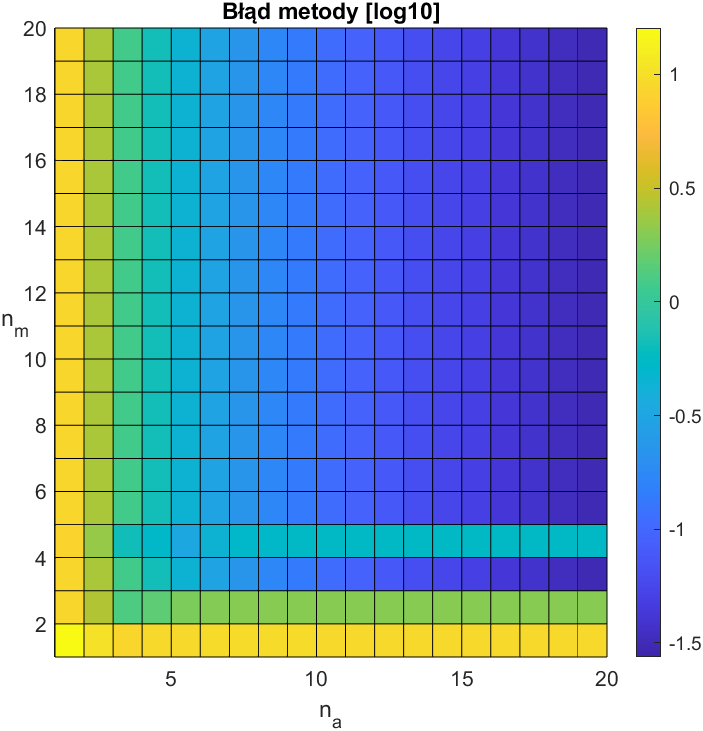
\includegraphics[height=7cm]{error.png}
    \caption{Średni błąd przybliżenia całki 4 stopnia, w zależności od liczby podziałów modułu ($n_m$) oraz liczby podziałów argumentu ($n_a$).}
\end{figure}

\begin{figure}[h]
    \centering
    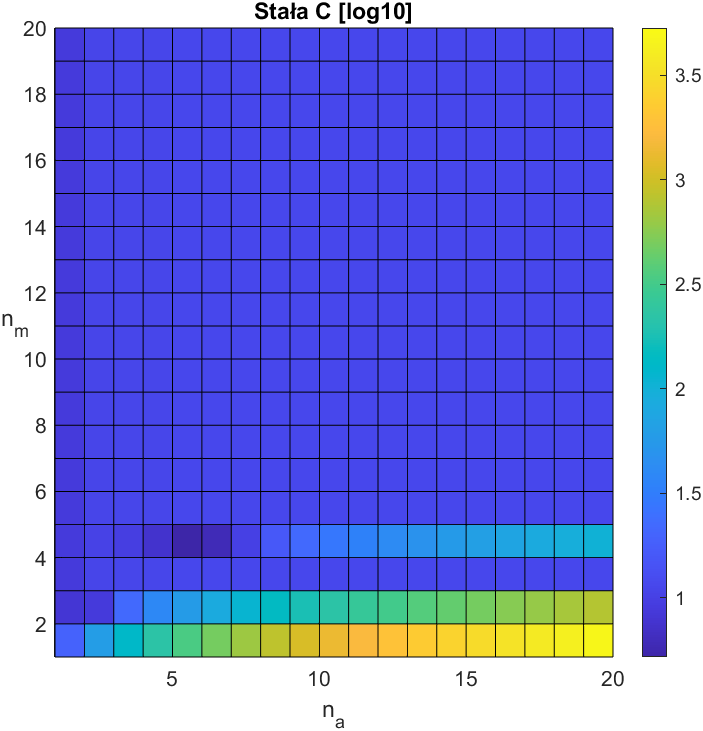
\includegraphics[height=7cm]{stalaC.png}
    \caption{Stała $C$ oszacowana poprzez $E(f)\cdot n_m^2$, dla dużych $n_m, n_a$ $C(i,j)=const$.}
\end{figure}

    Dodatkowym problemem badanej metody są błędne przybliżenia dla małych wartości $n_a, n_m$, błąd względny rzędu $80\%$, jest to spowodowane nierównomiernym rozkładem węzłów kwadratury, w Dodatku zostaną zaproponowane metody rozwiązania tego problemu w celu zwiększenia dokładności metody.

\break

\section*{Dodatek}
    Dodatek skupia się na modyfikacjach metody celem zmniejszenia błędu przybliżenia poprzez optymalizację rozkładu węzłów. 
        
\begin{figure}[h]
    \centering
    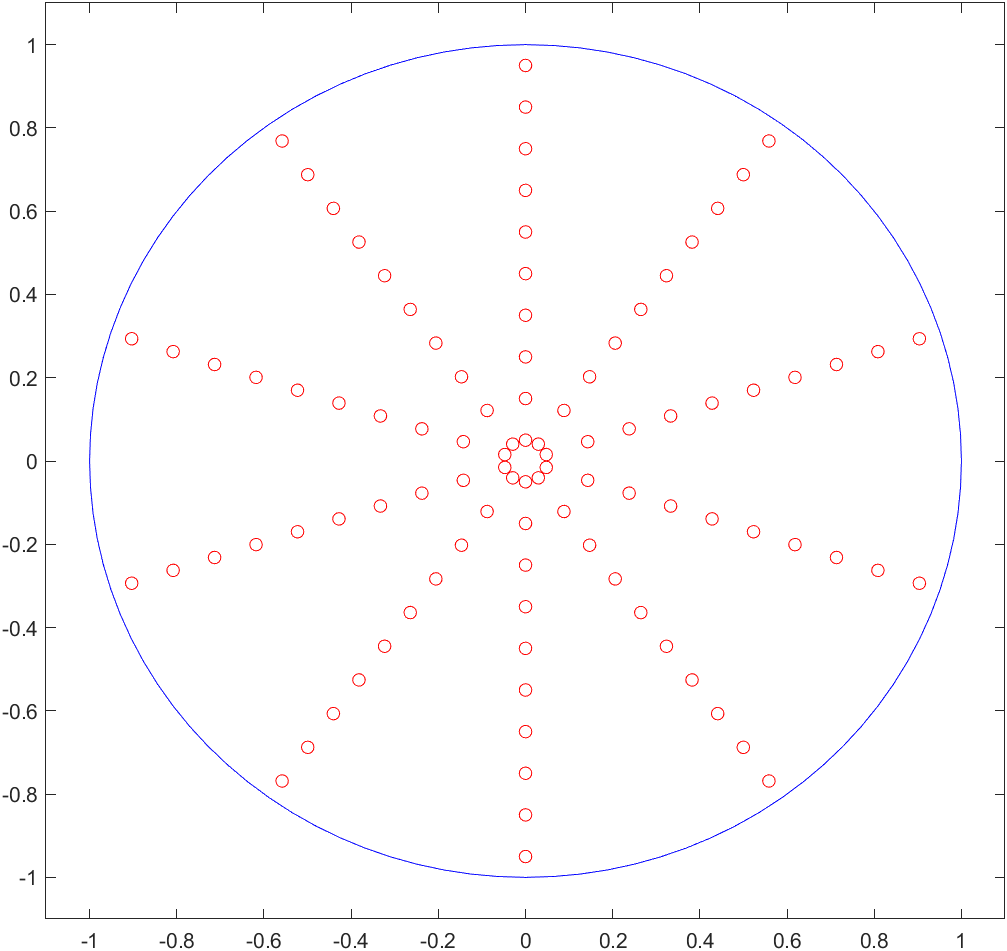
\includegraphics[height=5cm]{regular.png}
    \caption{Rozkład węzłów przy $n_a=10$ oraz $n_m=10$}
\end{figure}

\section*{Modyfikacje metody}
\subsection*{Modyfikacja 1}
    Celem tej modyfikacji jest wyeliminowanie nierównomierności rozkładu węzłów wraz ze wzrostem odległości od środka obszaru całkowania.
    Niech $P_n$ oznacza pole n-tego pierścienia, otrzymujemy $P_n=\pi\Delta r^2(n^2-(n-1)^2)=\pi\Delta r^2(2n-1)$, stąd dzieląc $P_n$ na $2n-1$, lub wielokrotność, podzbiorów otrzymujemy podział koła na podzbiory o równym polu.
    
\subsection*{Modyfikacja 2}
    Ta modyfikacja eliminuje problem nierównomiernego rozkładu poprzez zmienna długość podziałów $r$.
    Niech $r_n$ oznacza szerokość n-tego pierścienia.
    Z $P_1=P_2=...=P_n$, oraz $\sum\limits_{i=1}^n{P_n}=1$, otrzymujemy $r_1^2=r_2^2-r_1^2=...=r_n^2-r_{n-1}^2$ oraz $r_n=1$, co daje $r_n=\sqrt{\frac{n}{N}}$, gdzie $N$ oznacza liczbę podziałów długości promienia.
    
\subsection*{Modyfikacja 3}
    Modyfikacja łączy pomysły dwóch poprzednich, a więc korzysta ze zmiennej długości podziałów promienia oraz rosnącej liczby węzłów na każdym kolejnym pierścieniu.
    
\begin{multicols}{3}
    \small
    \centering
    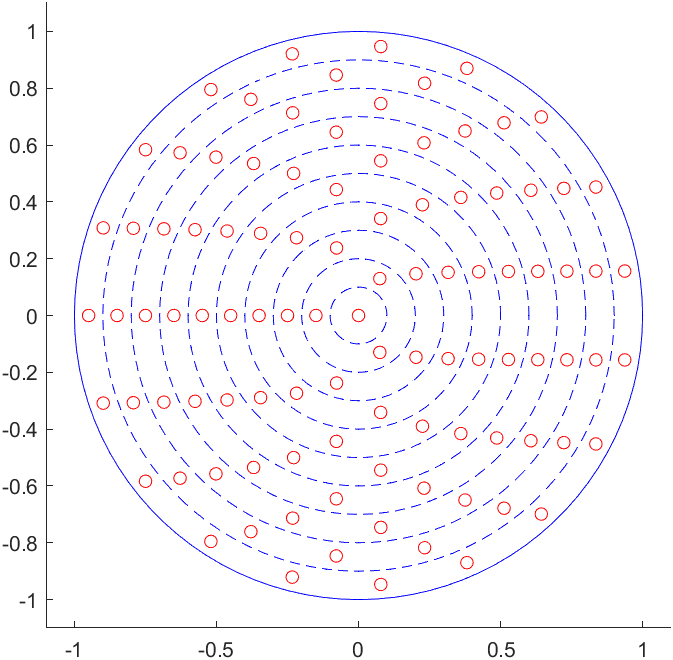
\includegraphics[height=5cm]{mod1.png}
     \small
    Modyfikacja 1.
    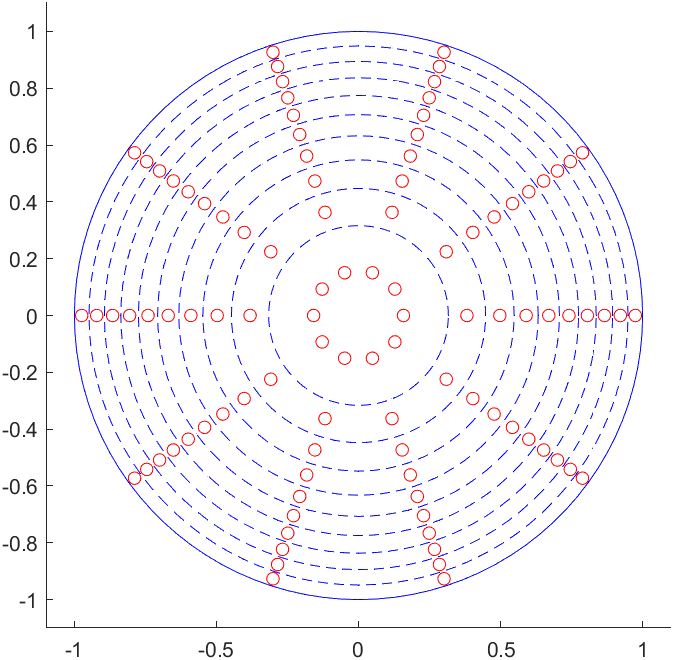
\includegraphics[height=5cm]{mod2.png}
     \small
    Modyfikacja 2.
    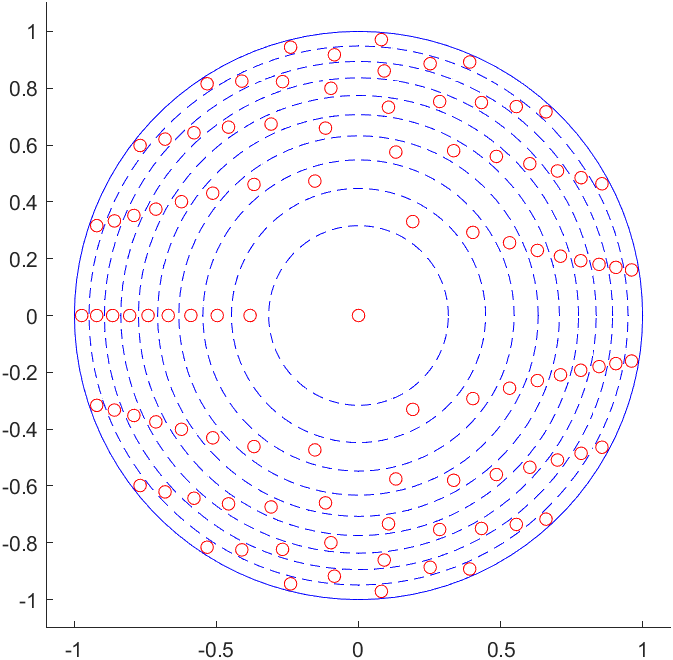
\includegraphics[height=5cm]{mod3.png}
     \small
    Modyfikacja 3.
\end{multicols}

\break

    Poniższy wykres przedstawia uśredniony błąd przybliżenia całek 4 stopnia (100 całek), w zależności od użytej metody. Parametr $A$ dla  metody 1. i 3. modyfikuje ilość węzłów w pierścieniu, na $n$-tym pierścieniu znajduje się $A\cdot(2n-1)$ węzłów, stąd metody 1. i 3. dla danego $A$ oraz $M$ opiera się na $A\cdot M^2$ węzłach, gdzie $M$ to ilość podziałów modułu liczby.
    
\begin{multicols}{3}
    \small
    \centering
    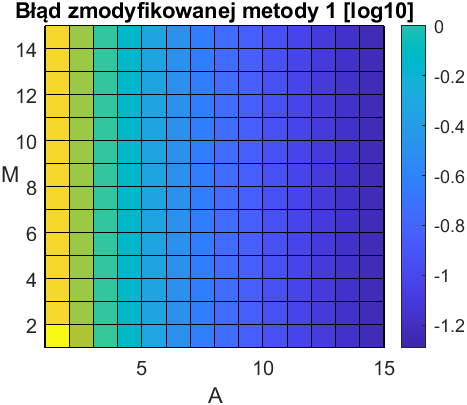
\includegraphics[height=5cm]{blad1.png}
     \small
    Modyfikacja 1.
    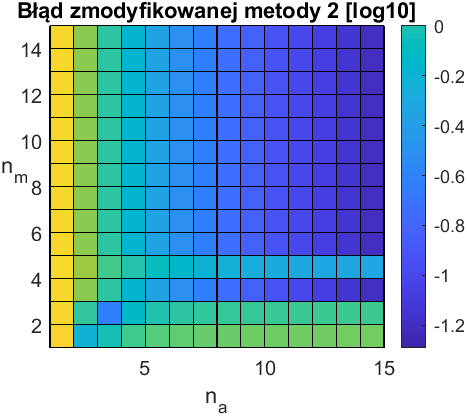
\includegraphics[height=5cm]{blad2.png}
     \small
    Modyfikacja 2.
    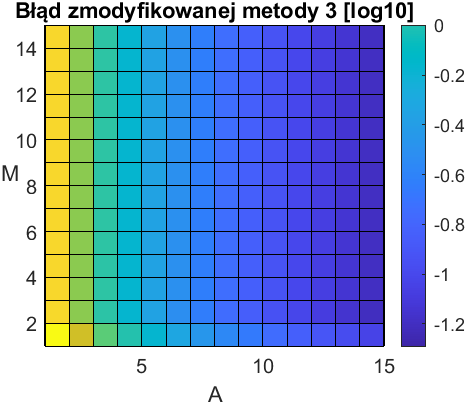
\includegraphics[height=5cm]{blad3.png}
     \small
    Modyfikacja 3.
\end{multicols}

    Oszacowana została również stała C, przybliżająca błąd metody. Dla kolejnych metody odpowiednio $8,49$, $6,96$, $6,8$. Zatem modyfikacja 2. przy najmniejszej ilości obliczeń zapewnia najdokładniejsze przybliżenie, jednak dla wartości $n_a\leq 6$ oraz $n_m\leq 6$ błąd jest zdecydowanie większy. 

\end{document}
